\documentclass[a4paper]{article}\usepackage[dvips]{graphicx}

\begin{document}

\begin{center}
{\Large NeXus Application Definitions Tutorial }\\
Mark K\"onnecke\\
Version: March 2009\\
\end{center}


\section{Introduction }

NeXus is a data exchange format for scientists working in the field of neutron or xray scattering and 
muSR spectroscopy. This document is a guide for people who wish to apply the NeXus data format to 
their problem: be it the definition of a raw dat format for an instrument or an exchange format for some
form of preprocessed data. This document assumes that the reader has some knowledge about the NeXus 
data format. More information about NeXus can be found at the NeXus web site at: www.nexusformat.org 


Let us start with a recapitulation of some of NeXus feautures which are relevant for application 
definitions. NeXus experts can skip this section. The first are some of the NeXus guiding principles.


\begin{itemize}\item A NeXus file has to contain all the data necessary for standard data analysis.
\item A NeXus file is extendable.
\end{itemize}

Then data in NeXus files is stored in a structured form. To this purpose NeXus uses the concept of groups. Groups 
are containers which can contain other groups or data sets. NeXus identifies groups through two attributes: group names 
and the groups class. NeXus makes no assumptions about  group names. They are free. This is different for classes: 
class names are part of the NeXus standard and always start with the prefix NX.  At first glance this scheme seems odd.
After all, a data analysis program becomes much easier to write if all the names would be known in advance. However, 
there is a good reason for the name/class scheme and this is the fact that multiple elements of the same type may 
occurr. A reflectometer has many slits of type NXaperture. Lots of instruments have multiple detector banks of
 type NXdetector. A data analysis program has to figure that out and ask: Hey dude which data shall I evaluate? 
 


A NeXus file has the following structure:


\begin{itemize}\item NXentry
\begin{itemize}\item NXuser
\item NXmonitor
\item NXsample
\item NXdata
\item NXinstrument
\begin{itemize}\item NXcomponent
\item NXcomponent
\end{itemize}\end{itemize}\end{itemize}This means that at the root level of a NeXus file are one or more groups of type NXentry. These are NeXus support for 
storing multiple related data sets in one file. The NXentry group contains further groups:


\begin{itemize}\item one or more NXuser groups containing information about the experimenter
\item An NXsample group which contains data about the sample
\item One or more NXmonitor groups which contains data about the counting statistics and how counting happened.
\item An NXinstrument which contains further groups, one for each relevant instrument component.
\item One or more NXdata groups. These groups are only there to facillitate automatic plotting. These groups 
 are to contain a summary of the data necessary to create a default plot of the data in the file.
\end{itemize}

A word about coordinate systems: NeXus supports two: if you need to be very exact, use the McStas coordinate system. 
This is mostly of interest to simulators wishing to store the results of simulations in NeXus files. Most people will use the 
simple coordinate system as shown in figure 1. 


\begin{figure}[!ht]
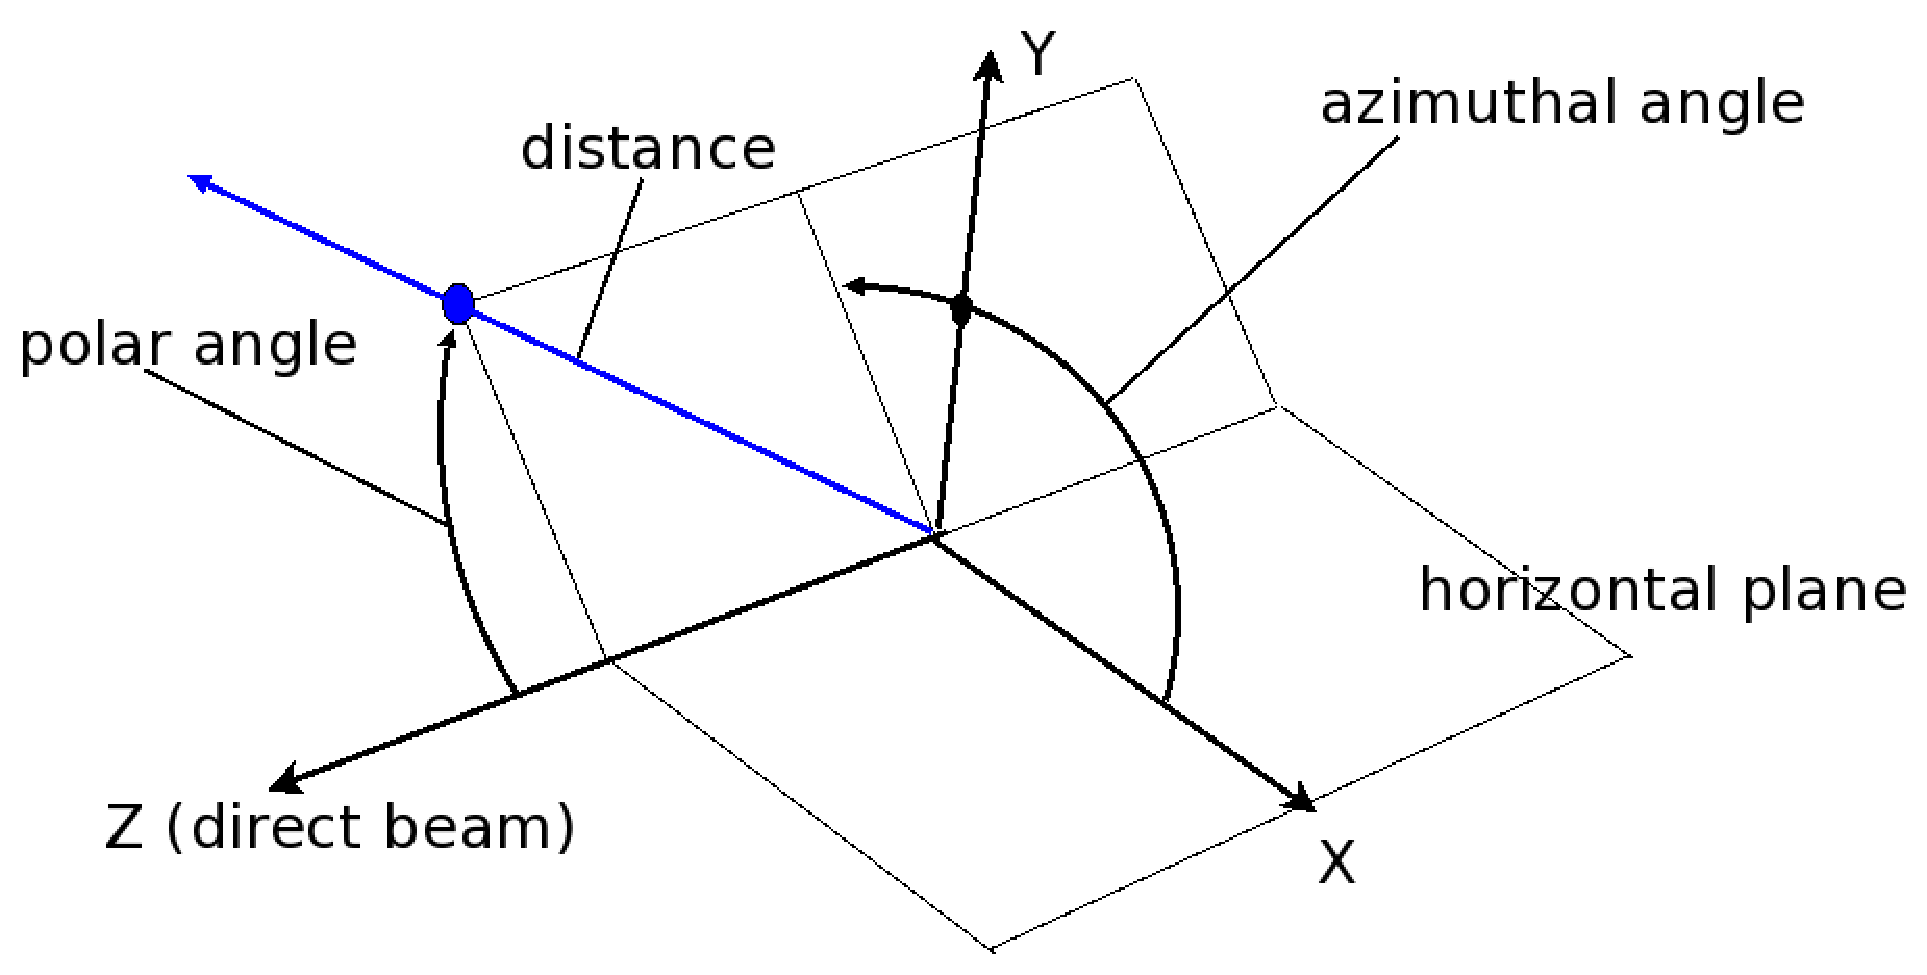
\includegraphics[width=0.75\textwidth]{polplane.eps}
\label{fig1}
\caption{NeXus Coordinate Systems} 
\end{figure}



This looks complicated but becomes very simple if the instrument does not move out of the scattering plane: Then the 
NeXus polar\_angle becomes what is commonly known as two theta. There is another gotcha: NeXus stores the polar\_angle 
downstream: for example if you have a monochromator pointing at a sample, the polar\_angle of the monochromator is 
stored at the sample. The NIAC decided upon this after lengthy discussions because it is the only way how to cope with 
instruments which have multiple backends, like multiple analysers.  
The zero point for distances is the sample. Distances are in relation to this zero point. negative distances point 
towards the source, positive distances behind the sample.



It is useful to come clear about some terms:


\begin{description}
\item[base classes]  are dictionaries of names to use for the various data items in a NeXus group. Consequently there is 
 a base class for each defined NeXus groups.  Base classes define names for anything which can possibly be used 
 to describe this component. Thus base classes tend to be pretty big. Do not worry, we reduce this later.
\item[application definition]  This is a definition of the content of a NeXus file as used for a special instrument type or 
 an exchange format for data later in the data analysis pipeline. This content is what a NeXus file producer has to 
 provide in order to write a valid NeXus file for this type of application. In turn a data analysis software author can 
 rely on this information to be present in a valid NeXus file for this type of application. Another view on an application 
 definition to see it as an interface or a contract between the producer and the consumer about what the file has to 
 contain to be useful.   
\end{description}

NeXus base class and application definitions are written in NeXus Definition Language, NXDL. NXDL is in fact an 
application of XML to the problem of writing application definitions. The nice thing about NXDL is that it can be 
converted to an XML schema which then can be used to validate NeXus file against the definition. 




\section{Before you Start }

Before considering to start with an application definition, verify that no existing application definition 
is published on the NeXus web site which fits your problem. If so, USE IT, that is what standards are for. If there 
is something you do not like about the existing application definition, feel free to discuss your 
concern with the NIAC. 


Before you can start with writing NeXus application definitions you need two implements:


\begin{itemize}\item A copy of the current NeXus base classes and application definitions for reference.
\item An XML editor
\end{itemize}
A copy of the current NeXus definitions will be made available for download from the NeXus web site. 
Until then, ask any NIAC member to provide you with a kit.


The XML editor is really your choice. There are many good ones out  there. It is advantageous if the XML 
editor support XML schema. This because a XML schema for NXDL is provided by the NeXus group and with 
this schema your XML editor can help you to create a valid NXDL file and make suggestions what  can be 
legally entered at the various places in the NXDL file you are authoring. A suitable free XML editor is the one 
coming with the WWW-tools  plugin for the eclipse development framework.



\section{The Tutorial Setup }

Consider yourself to be in a position at the HYpothetical NEw Source (HYNES).  You are tasked to write an 
application definition for raw data from the WOnderful New Instrument (WONI). This being a tutorial WONI is actually a simple 
powder diffractometer. See the schema in figure 2.
\begin{figure}[!ht]
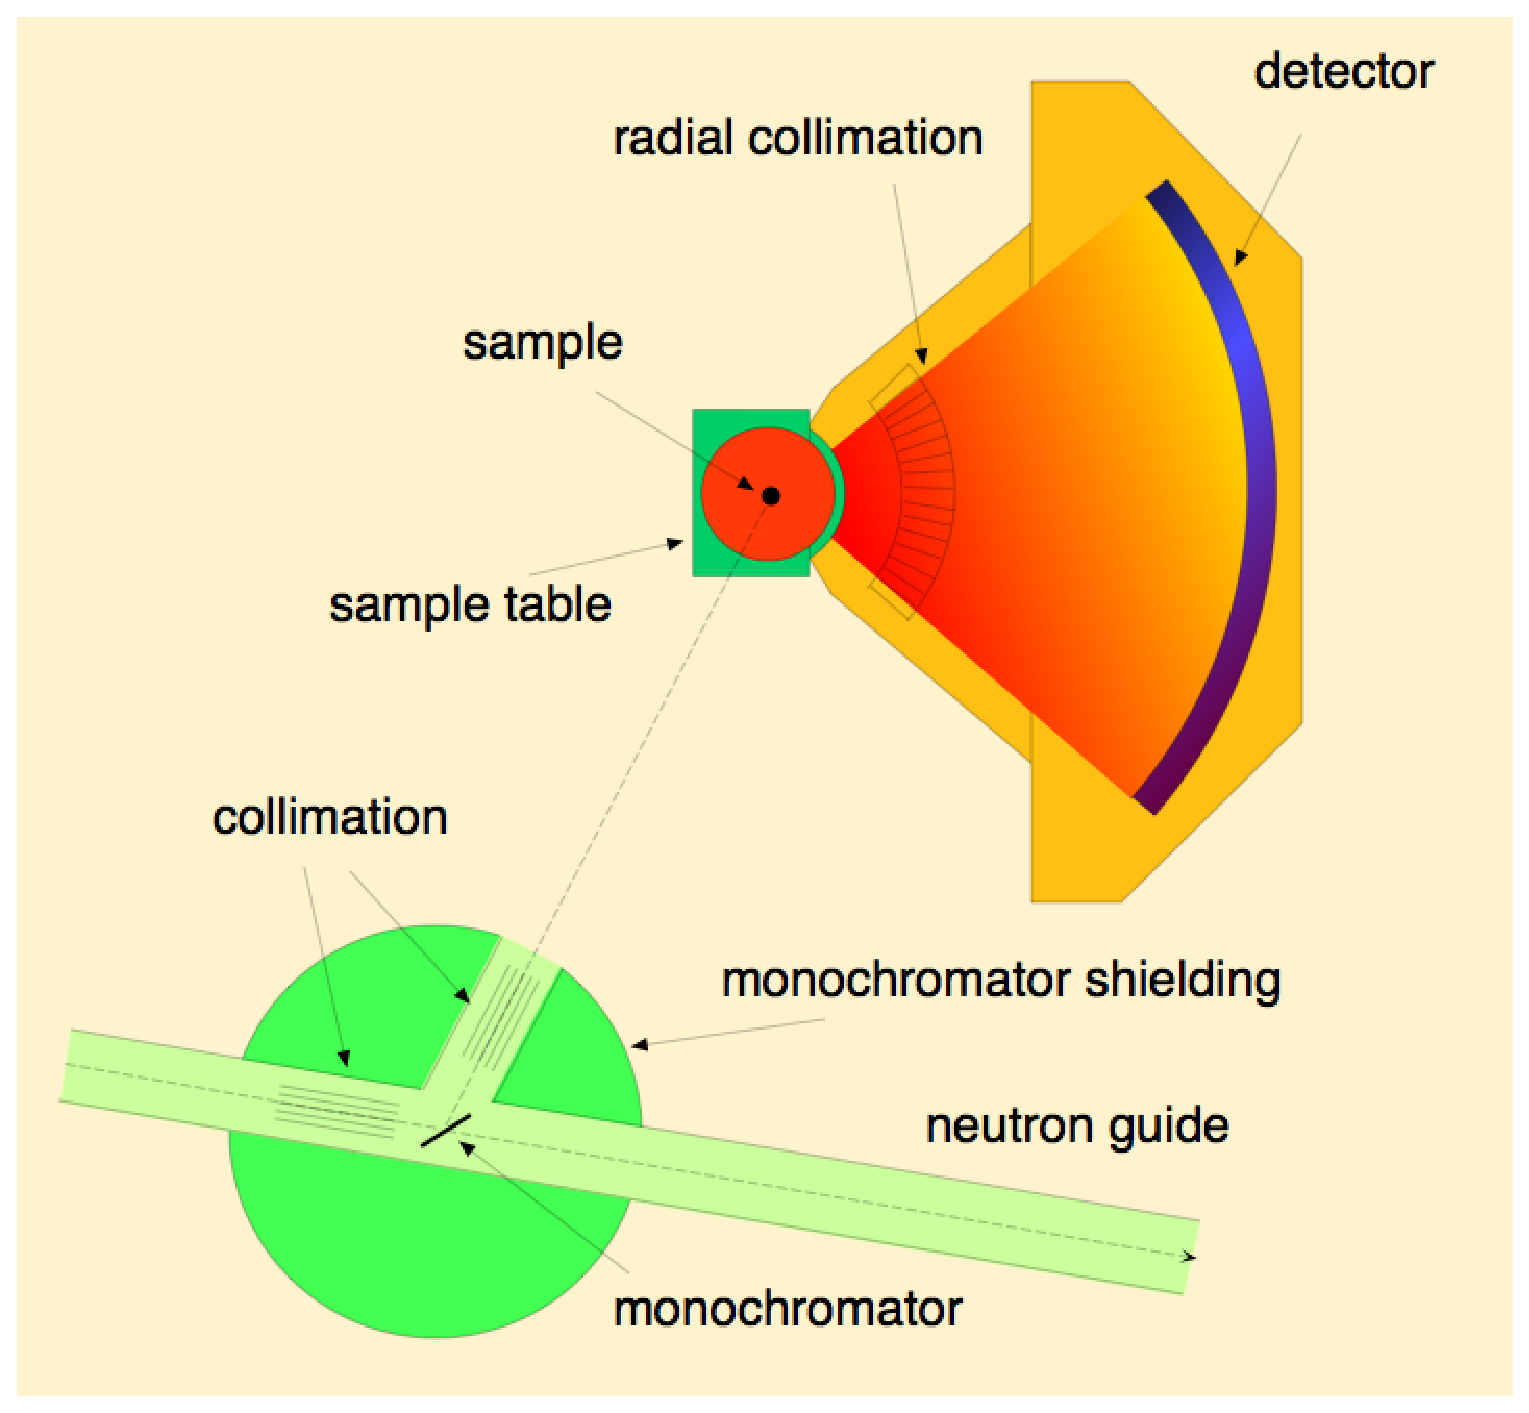
\includegraphics[width=0.75\textwidth]{dmc.eps}
\label{fig2}
\caption{The WONI example powder diffractometer}
\end{figure}



So there is a monochromator which generates a monochromatic beam which hits the 
sample which diffracts the beam. And the diffracted beam is collected in a large banana shaped position sensitive detector. 
Typical data looks like figure 3. 
\begin{figure}[!ht]
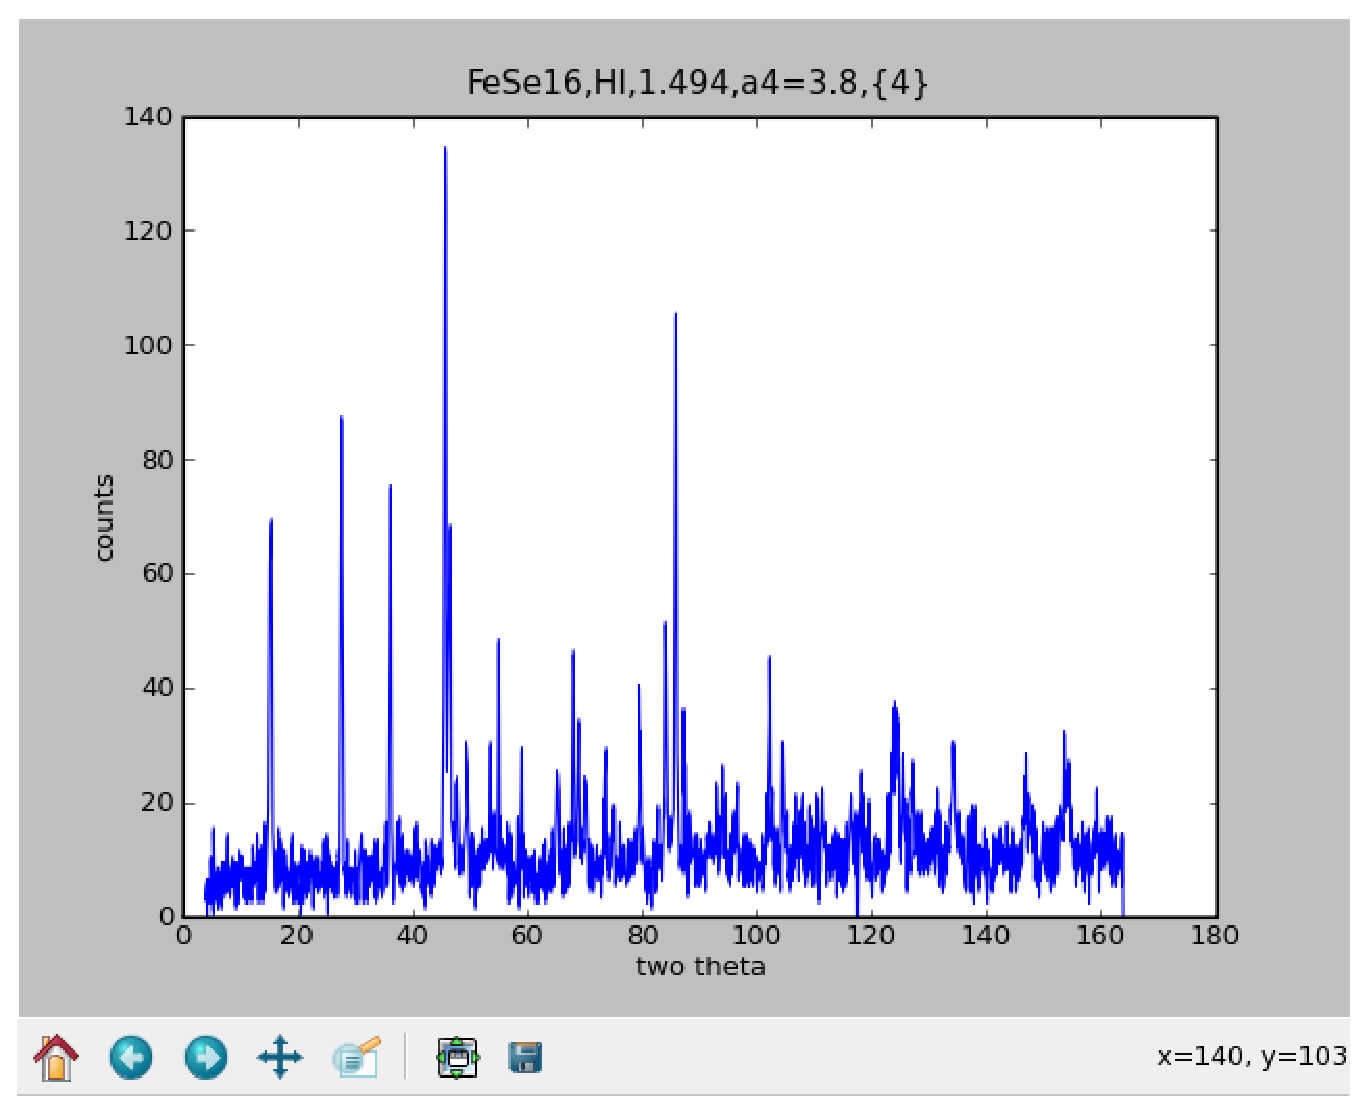
\includegraphics[width=0.75\textwidth]{powderimage.eps}
\label{fig3}
\caption{Example Powder Diffraction Plot}
\end{figure}


You have a generous background plus quite a number of peaks on it.




\section{Application Definition Steps }

With all this introductory stuff out of the way, let us look at the process required to define an application definition:


\begin{enumerate}\item {\em  Think!} hard about what has to go into the data file.
\item {\em  Map} the required data items into the NeXus file structure
\item {\em  Cast} this mapping into a NXDL file
\item {\em  Standardize} your definition through communication with the NIAC. 
\end{enumerate}

\section{Step 1: Think! about Data }

This is actually the hard bit. There are two things to consider:


\begin{enumerate}\item What has to go into the data file
\item What is the normal plot for this type of data.
\end{enumerate}For the first part, one of the NeXus guiding principles gives us - Guidance!


\begin{quote}

A NeXus file has to contain all the data necessary for standard data analysis.


\end{quote}

Not more and not less for an application definition. What is standard data analysis or a standard plot 
of course depends on the application type. Consult senior scientists in you field about this is if you are 
unsure. May be you must call an international meeting with domain experts to haggle that out. When considering 
this people tend to put in everything which might come up. This is not the way to go. The filter is: is this data 
item necessary for common data analysis. And only these data items belong into an application definition. The purpose 
of an application definition is that an author of upstream software who consumes the file can expect certain data items 
to be there at  well defined places. On the other hand if there is a development in your field which analyses data 
in a novel way and requires more data to do it: then it is better to err towards the side of more data. 


Now for the case of WONI the standard data analysis is either rietveld refinement or profile analysis. For both puposes 
the kind of probe,  the wavelength, the monitor (which tells us how long we counted for),
  the counts and the two theta angle of each detector element is required. Usually 
it is also desirable to know what is being analysed, so some meta data would be nice: a title, the sample name and the 
sample temperature. The data typically being plotted is two theta against counts, as shown above. Summing it up the 
following information is required.


\begin{table}[!ht]
\begin{tabular}{|c|c|}
\hline
 title\\ \hline
sample name\\ \hline
sample temperature\\ \hline
monitor\\ \hline
probe\\ \hline
wavelength\\ \hline
two theta of detector elements\\ \hline
counts for each detector element\\ \hline
\end{tabular}
\end{table}
If you start to worry that this is to little information, hold on, the section on Using an Application Definition, will 
reveal the secret how to go from an application definition to a practical file.




\section{Step 2: Map Data into the NeXus Hierarchy }

This step is actually easier then the first one. We need to map the data items which were collected in Step 1 into the 
NeXus hierarchy. A NeXus file hierarchy starts with an NXentry group. At this stage it is advisable to pull up the base class 
definition for NXentry and study it. The first thing you might notice is that NXentry contains a field named title. Reading the 
documentaion you quickly realize that this is a good place to store our title in. So the first mapping has been found.


\begin{center}

 {\em  title = /NXentry/title}


\end{center}

These mapping descriptions just contain the path strings into the NeXus file with the class names of the groups to use.   


Another thing to notice in the NXentry base class is the existence of a group of class NXsample. This looks like a great 
place to store information about the sample. Studying the NXsample base class confirms this view and there are two new mappings:


\begin{center}

 {\em  sample name  =  /NXentry/NXsample/name} \linebreak
 {\em  sample temperature  = /NXentry/NXsample/temperature}


\end{center}

Scanning the NXentry base class some more reveals that there can be a NXmonitor goup at this level. Looking up the base 
class for NXmonitor reveals that this is the place to store our monitor information.


\begin{center}
 
 {\em  monitor = /NXentry/NXmonitor/data}


\end{center}


For the other data items, there seem to be no solutions in NXentry. But each of these data items describe the instrument in more 
detail. NeXus stores instrument descriptions in the /NXentry/NXinstrument branch of the hierarchy. Thus we continue by looking at 
the definition of the NXinstrument base class. In there we find further groups for all possible instrument components. Looking at the 
schematic of WONI we realize that there is a source, a monochromator and a detector. Suitable groups can be found for this in 
NXinstrument and further inspection of the appropriate base classes reveals the following further mappings:


\begin{center}

 {\em  probe = /NXentry/NXinstrument/NXsource/probe} \linebreak
 {\em  wavelength = /NXentry/NXinstrument/NXcrystal/wavelength} \linebreak
 {\em  two theta of detector elements = /NXentry/NXinstrument/NXdetector/polar\_angle}\linebreak
 {\em  counts for each detector element = /NXentry/NXinstrument/NXdetector/data}


\end{center}


Thus we mapped all our data items into the NeXus hierarchy! What still needs to be done is to decide upon the content of the NXdata 
group in NXentry. This group is supposed to hold the data necessary to make a quick plot of the data. For WONI this is counts versus 
two theta. Thus we add this mapping:


\begin{center}

 {\em  two theta of detector elements = /NXentry/NXdata/polar\_angle}\linebreak
 {\em  counts for each detector element = /NXentry/NXdata/data}\linebreak


\end{center}

The full mapping is documented in table 2.


\begin{table}[!ht]
\begin{tabular}{|c|c|c|}
\hline
 title&/NXentry/title\\ \hline
sample name &/NXentry/NXsample/name\\ \hline
sample temperature &/NXentry/NXsample/temperature\\ \hline
monitor&/NXentry/NXmonitor/data\\ \hline
probe&/NXentry/MXinstrument/NXsource/probe\\ \hline
wavelength&/NXentry/MXinstrument/NXcrystal/wavelength\\ \hline
two theta of detector elements&/NXentry/NXinstrument/NXdetector/polar\_angle\\ \hline
counts for each detector element&/NXentry/NXinstrument/NXdetector/data\\ \hline
two theta of detector elements&/NXentry/NXdata/polar\_angle\\ \hline
counts for each detector element&/NXentry/NXdata/data\\ \hline
\end{tabular}
\end{table}Looking at this one might get concerned that the two theta and counts data is stored in two places and 
thus duplicated. Stop worrying, this problem is solved at the NeXus API level. Typically NXdata will only hold links 
to the corresponding data items in /NXentry/NXinstrument/NXdetector.



In this step problems might occur. The first is that the base class definitions contain a bewildering number of parameters. 
This is on purpose: the base classes serve as dictionaries which define names for everything which possibly can occurr. You do 
not have to give all that information. The filter is, as already said, what is required for typical data analysis for this type of 
application. You might also be unsure how to correctly store a particular data item. In such a case contact the NIAC for help.
Another problem which can occur is that you require to store information for which there is no name in one of 
the existing base classes or you have a new instrument component for which there is no base class alltogether. In such a case, 
please feel free to contact the NIAC with a suggestion for an extension of the base classes in question.




\section{Step 3: Cast your Mapping into a NXDL File }

This is even easier. Some XML editing is necessary. Fire up your XML editor of choice and open a file. 
If your XML editor support XML schema, it is worth to load nxdl.xsd. Now your XML editor can help you to 
create a proper NXDL file. As always, the start is an empty template file. This looks like this:


\begin{verbatim}

<?xml version="1.0" encoding="UTF-8"?>
<!--
# NeXus - Neutron and X-ray Common Data Format
# 
# Copyright (C) 2008-2011 NeXus International Advisory Committee (NIAC)
# 
# This library is free software; you can redistribute it and/or
# modify it under the terms of the GNU Lesser General Public
# License as published by the Free Software Foundation; either
# version 3 of the License, or (at your option) any later version.
#
# This library is distributed in the hope that it will be useful,
# but WITHOUT ANY WARRANTY; without even the implied warranty of
# MERCHANTABILITY or FITNESS FOR A PARTICULAR PURPOSE.  See the GNU
# Lesser General Public License for more details.
#
# You should have received a copy of the GNU Lesser General Public
# License along with this library; if not, write to the Free Software
# Foundation, Inc., 59 Temple Place, Suite 330, Boston, MA  02111-1307  USA
#
# For further information, see http://www.nexusformat.org

########### SVN repository information ###################
# $Date: 2009-01-16 20:21:39 +0100 (Fri, 16 Jan 2009) $
# $Author: Mark Koennecke $
# $Revision: 261 $
# $HeadURL: https://svn.nexusformat.org/definitions/trunk/applications/NXmonopd.xml $
# $Id: $
########### SVN repository information ###################
-->
<nx:definition name="" extends="" type="group" 
 xmlns:nx="http://definition.nexusformat.org/schema/3.1" 
 xmlns:xsi="http://www.w3.org/2001/XMLSchema-instance" 
  xsi:schemaLocation="http://definition.nexusformat.org/schema/3.1 ../nxdl.xsd ">

</nx:definition>
\end{verbatim}
 
This is just the basic XML for a NXDL definition. It is advisable to change some of 
the documentation strings. 


The next thing which needs to be done is adding groups into the definition. A group is 
define by some XML like this:


\begin{verbatim}

<group type=" NXdata">

</group>
\end{verbatim}
 
The type is the actual NeXus base class this group belongs to. Optionally a name attribute may be 
given.


Then one needs to include data items too. The XML for such a data item looks like this:


\begin{verbatim}

<field name="polar_angle" type="NX_FLOAT units="NX_ANGLE"">
  <doc>Link to polar angle in /NXentry/NXinstrument/NXdetector</doc>
  <dimensions size="1">
    <dim index="1" value="ndet"/>
  </dimensions>
<field>
\end{verbatim}

The attribute name is self describing, the type can be looked up in the relevant base class 
definition. A field definition can optionally contain a doc element which contains a description of 
the data item. The dimensions entry specifies the dimensions of the data set. The size attribute in the 
dimensions tag sets the rank of the data, in the example 1. In the dimensions group there must be rank 
dim fields. Each dim tag holds two attributes: index determines to which dimension this tag belongs, the 1 means 
 the first dimension. The value attribute then describes the size of the dimension. These can be plain integers, 
variables, such as int the example ndet and expressions like tof+1. 
  


Thus a NXDL file can be constructed. The full NXDL file for the WONI example is given as an appendix.




\section{Step 4: Standardization }

Basically your are done: your first application definition for NeXus is constructed. In order to 
make your work a standard for that particular application type some more steps are required:


\begin{enumerate}\item Send you application definition to the NIAC for review
\item Correct your definition for the comments of the NIAC.
\item Cure and use the definition for a year
\item After a final review, it becomes the standard.
\end{enumerate}The NIAC does like to look at application definitions before they become a standard. The one year 
curation period is in place in order to gain practical experience with the definition. And to sort 
out bugs from Step 1.  In this period data shall be written and analysed in the new application definition. 




\section{Using an Application Definition }

The application definition is like an interface for your data file. In practice files will contain 
far more information. For this, the extendable capability of NeXus comes in handy. More data can be added, 
and upstream software relying on the interface defined by the application definition can still retrieve the 
necessary information  without any changes to their code.


NeXus application definitions only standardizes classes. You are free to decide upon names of groups. Please 
use sensible, descriptive names and separate multi worded names with underscores. 



Something most people whish to add is more meta data, for example in order to index files into a database 
of some sort. Go ahead, do so, if applicable scan the NeXus base classes for standardized names. For meta data, 
consider to use the NXarchive definition. In this context it is worth to mention that a practical NeXus file might 
adhere to more then one application definition. For example, WONI data files may adhere to the NXmonopd and NXarchive 
definition. The first for data analysis, the second for indexing into the database. 


Often, instrument scientists want to store the complete state of their instrument in data files in order to be able 
to find out what went wrong if the data is unsatisfactory. Go ahead, do so, please use names from the 
NeXus base classes.


Site policy might require you to store the names of all your bosses up to the current prime minister in 
data files. Go ahead, add as many NXuser classes as required to store that information. 


Your Scientific Accounting Department (SAD) may ask to store billing information into data files. Go ahead, 
do so, just do not expect the NIAC to provide base classes for this and do not use the prefix NX for 
your classes. 


In most cases, NeXus files will just have one NXentry class group. But it may be required to store multiple related data 
sets of the results of data analysis into the same data file. In this case create more entries. Each entry should be 
interpretable standalone, i.e. contain all the information of a complete NXentry class. Please keep in mind that groups 
or data items which stay constant across entries can always be linked in.  



\section{Processed Data }

Data reduction and analysis programs are encouraged to store their results in NeXus data files. 
As far as the necessary, the normal NeXus hierarchy is to  be implemented. In addition processed 
data file must contain a NXprocess group. This group contains the name of the data processing program 
and the parameters used to run this program in order to achieve the results stored in this entry. Multiple 
processing steps must have a separate entry each. 



\section{Appendix A: The NXmonopd Definition }

\begin{verbatim}

<?xml version="1.0" encoding="UTF-8"?>
<!--
# NeXus - Neutron and X-ray Common Data Format
# 
# Copyright (C) 2008 NeXus International Advisory Committee (NIAC)
# 
# This library is free software; you can redistribute it and/or
# modify it under the terms of the GNU Lesser General Public
# License as published by the Free Software Foundation; either
# version 3 of the License, or (at your option) any later version.
#
# This library is distributed in the hope that it will be useful,
# but WITHOUT ANY WARRANTY; without even the implied warranty of
# MERCHANTABILITY or FITNESS FOR A PARTICULAR PURPOSE.  See the GNU
# Lesser General Public License for more details.
#
# You should have received a copy of the GNU Lesser General Public
# License along with this library; if not, write to the Free Software
# Foundation, Inc., 59 Temple Place, Suite 330, Boston, MA  02111-1307  USA
#
# For further information, see http://www.nexusformat.org

########### SVN repository information ###################
# $Date: 2009-03-04 07:10:14 +0100 (Wed, 04 Mar 2009) $
# $Author: Pete Jemian $
# $Revision: 334 $
# $HeadURL: https://svn.nexusformat.org/definitions/trunk/applications/NXmonopd.nxdl.xml $
# $Id: NXmonopd.nxdl.xml 334 2009-03-04 06:10:14Z Pete Jemian $
########### SVN repository information ###################
-->
<definition xmlns="http://definition.nexusformat.org/nxdl/3.1" xmlns:xsi="http://www.w3.org/2001/XMLSchema-instance" name="NXmonopd" extends="NXobject" type="group" xsi:schemaLocation="http://definition.nexusformat.org/nxdl/3.1 ../nxdl.xsd " svnid="$Id: NXmonopd.nxdl.xml 334 2009-03-04 06:10:14Z Pete Jemian $">
    <doc> Monochromatic Neutron and X-Ray Powder Diffraction. Instrument definition for a powder
        diffractometer at a monochromatic neutron or X-ray beam. This is both suited for a powder
        diffractometer with a single detector or a powder diffractometer with a position sensitive
        detector. </doc>
    <group type="NXentry">
        <field name="title"/>
        <field name="start_time" type="NX_DATE_TIME"/>
        <field name="end_time" type="NX_DATE_TIME"/>
        <group type="NXinstrument">
            <group type="NXsource">
                <field name="type"/>
                <field name="name"/>
                <field name="probe">
                    <enumeration>
                        <item value="neutron"/>
                        <item value="x-ray"/>
                        <item value="electron"/>
                    </enumeration>
                </field>
            </group>
            <group type="NXcrystal">
                <field name="wavelength" type="NX_FLOAT" units="NX_LENGTH">
                    <doc>Optimum diffracted wavelength</doc>
                    <dimensions size="1">
                        <dim index="1" value="i"/>
                    </dimensions>
                </field>
            </group>
            <group type="NXdetector">
                <field name="polar_angle" type="NX_FLOAT">
                    <doc>where ndet = number of detectors</doc>
                    <dimensions size="1">
                        <dim index="1" value="ndet"/>
                    </dimensions>
                </field>
                <field name="data" type="NX_INT">
                    <dimensions size="1">
                        <dim index="1" value="ndet"/>
                    </dimensions>
                </field>
                <field name="efficiency" type="NX_FLOAT">
                    <doc>efficiency of each detecor</doc>
                    <dimensions size="1">
                        <dim index="1" value="ndet"/>
                    </dimensions>
                </field>
            </group>
        </group>
    </group>
    <group type="NXsample">
        <field name="name">
            <doc>Descriptive name of sample</doc>
        </field>
        <field name="rotation_angle" type="NX_FLOAT" units="NX_ANGLE">
            <doc> Optional rotation angle for the case when the powder diagram has been obtained
                through an omega-2theta scan like from a traditional single detector powder
                diffractometer </doc>
        </field>
    </group>
    <group type="NXmonitor">
        <field name="mode">
            <doc>Count to a preset value based on either clock time (timer) or received monitor
                counts (monitor).</doc>
            <enumeration>
                <item value="monitor"/>
                <item value="timer"/>
            </enumeration>
        </field>
        <field name="preset" type="NX_FLOAT">
            <doc>preset value for time or monitor</doc>
        </field>
        <field name="integral" type="NX_FLOAT" units="NX_ANY">
            <doc>Total integral monitor counts</doc>
        </field>
    </group>
    <group type="NXdata">
        <field name="polar_angle" type="NX_FLOAT">
            <doc>Link to polar angle in /NXentry/NXinstrument/NXdetector, ndp = number of detectors or data points</doc>
            <dimensions size="1">
                <dim index="1" value="ndp"/>
            </dimensions>
        </field>
        <field name="data" type="NX_INT">
            <doc>Link to data in /NXentry/NXinstrument/NXdetector</doc>
            <dimensions size="1">
                <dim index="1" value="ndp"/>
            </dimensions>
        </field>
    </group>
</definition>

\end{verbatim}
  






















\end{document}

